\subsection{\forlnameref Casos de uso}
\label{sec:useCases}

Se presenta a continuación la descripción de cada caso de uso por cada agrupación funcional referida en el punto anterior. Para simplificar el modelo, en todo momento se considera que la acción \textit{Buscar} conlleva a una posterior consulta de alguno de los elementos buscados.

\begin{shaded}
Se incluye una agrupación funcional completa de ejemplo, que ilustra los casos de uso \ac{CRUD}.
\end{shaded}

\subsubsection*{Gestión de Permiso}

\begin{figure}[H]
\centering
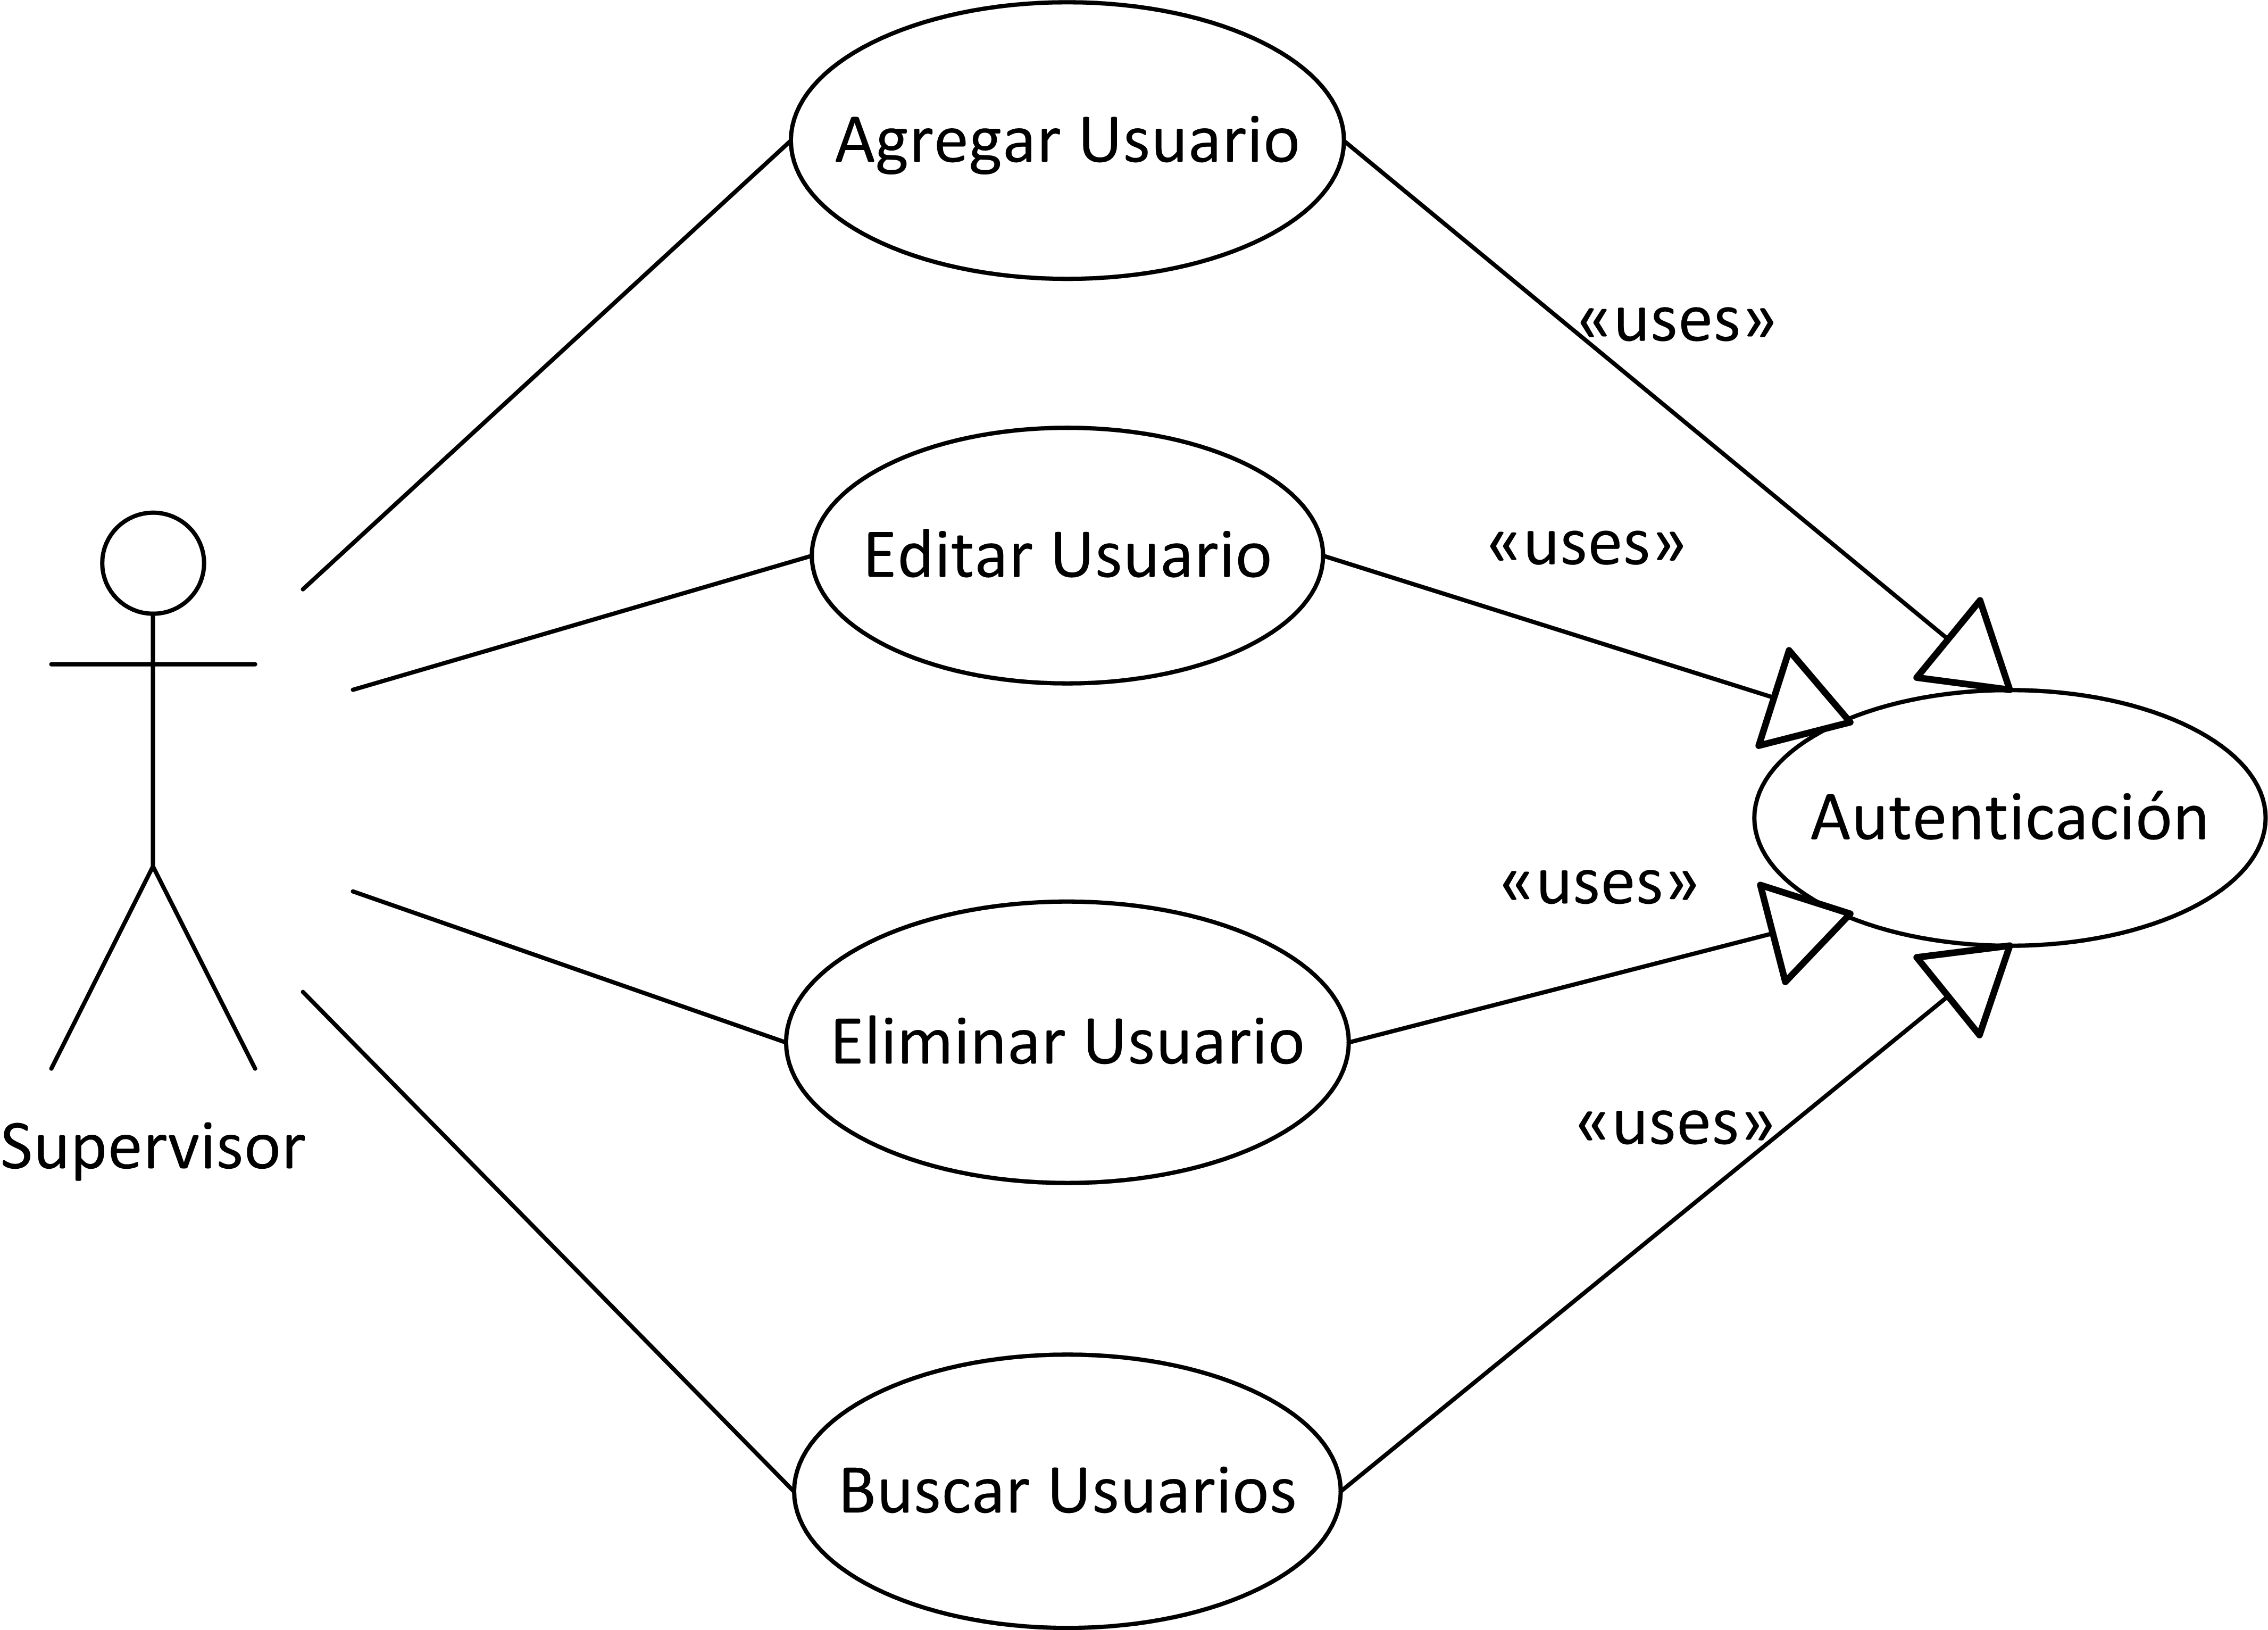
\includegraphics[scale=0.5]{usecasesAuths.png}
\caption{Diagrama de Casos de Uso de Gestión de Permiso}
\label{fig:usecasesAuths}
\end{figure}

% \begin{shaded}
% Si bien los diagramas de casos de uso son ilustrativos y permiten un vistazo general y estructurado de lo que hace el sistema, la descripción de los mismos pocas veces aporta algo al análisis, sobre todo en lo referente a los escenarios. Por ello y dado que aún sigue siendo práctica obligatoria en la carrera, se aconseja que se le dedique el menor tiempo posible al detalle de dichos escenarios, a excepción de que alguno siga una casuística más allá de las clásicas funciones de agregación, modificación, eliminación y búsqueda. Por otra parte, no es buena práctica referir explícitamente a ningún atributo de los requisitos de información. Es decir, en lugar de ``El \actor\ introduce el nombre, los apellidos y la edad'', es preferible ``El \actor\ introduce los datos''. Con eso se logran dos objetivos: en primer lugar, el no dedicarle tiempo innecesario; en segundo, y más importante, aislar en la medida de lo posible los requisitos de información de los casos de uso, de forma que una modificación en aquéllos no afecte a la descripción del proceso, obligando a hacer doble trabajo y aumentando la probabilidad de inconsistencia por error. No obstante, si hubiera algún dato con un tratamiento especial, sí sería necesario especificarlo en la descripción del caso de uso que lo contempla.
% \end{shaded}


\def \ucName {Autenticación}
\def \ucDescription {El \actor\ se autentifica en el sistema, previa comprobación de éste.}
\def \ucActors {Usuario}
\def \ucPreconditions {}
\def \ucMainScenery {
    \begin{ucscenery}
        \item[1.] El \sistema\ comprueba que el \actor\ está autentificado.
        \item[2.] El \sistema\ muestra el formulario.
        \item[3.] El \actor\ introduce los datos.
        \item[4.] El \actor\ acepta la acción.
        \item[5.] El \sistema\ comprueba que los datos son correctos.
        \item[6.] El \sistema\ registra al \actor\ como autentificado.
    \end{ucscenery}
}

\def \ucPostconditions {
    \begin{ucconditions}
        \item El \actor\ queda autentificado en el sistema.
    \end{ucconditions}
}
\def \ucAltSceneries {
    \begin{ucscenery}
        \item[1.a.] El \actor\ ya está registrado
        \begin{ucsubscenery}
            \item El \sistema\ cancela el caso de uso.
        \end{ucsubscenery}
        \item[5.a.] Hay un error en algún dato.
        \begin{ucsubscenery}
            \item El \sistema\ notifica el error.
            \item El \sistema\ vuelve al punto \textbf{2}.
        \end{ucsubscenery}
        \item[5.b.] El \sistema\ no puede acceder el modelo.
        \begin{ucsubscenery}
            \item El \sistema\ notifica el error.
            \item El \sistema\ vuelve al punto \textbf{2}.
        \end{ucsubscenery}
        \item[6.a.] El \sistema\ no puede modificar el modelo.
        \begin{ucsubscenery}
            \item El \sistema\ notifica el error.
            \item El \sistema\ vuelve al punto \textbf{2}.
        \end{ucsubscenery}
        \item[*.a.] El \actor\ cancela la acción.
        \begin{ucsubscenery}
            \item El \sistema\ cancela el caso de uso.
        \end{ucsubscenery}
    \end{ucscenery}
}
\def \ucNotes {}

\createUseCaseTable{tab:ucAddUser}
\def \ucName{Agregar Usuario}
\def \ucDescription {El \actor\ se registra en el sistema.}
\def \ucActors {Usuario (Técnico)}
\def \ucPreconditions {}
\def \ucMainScenery {
    \begin{ucscenery}
        \item[1.] El \sistema\ muestra el formulario de registro.
        \item[2.] El \actor\ introduce los datos.
        \item[3.] El \sistema\ comprueba que los datos son correctos.
        \item[4.] El \sistema\ registra al actor como una nueva entidad.
    \end{ucscenery}
}
\def \ucAltSceneries {
    \begin{ucscenery}
        \item[1.a.] No es posible autenticar al \actor.
        \begin{ucsubscenery}
            \item El \sistema\ cancela el caso de uso.
        \end{ucsubscenery}
        \item[5.a.] Los datos son incorrectos.
        \begin{ucsubscenery}
            \item El \sistema\ notifica el error.
            \item El \sistema\ vuelve al punto \textbf{3}.
        \end{ucsubscenery}
        \item[5.b.] La entidad ya existe en el sistema.
        \begin{ucsubscenery}
            \item El \sistema\ notifica el error.
            \item El \sistema\ vuelve al punto \textbf{3}.
        \end{ucsubscenery}
        \item[6.a.] El \sistema\ no puede modificar el modelo.
        \begin{ucsubscenery}
            \item El \sistema\ notifica el error.
            \item El \sistema\ vuelve al punto \textbf{3}.
        \end{ucsubscenery}
        \item[*.a.] El \actor\ cancela la acción.
        \begin{ucsubscenery}
            \item El \sistema\ cancela el caso de uso.
        \end{ucsubscenery}
    \end{ucscenery}
}
\def \ucNotes {}






% \createUseCaseTable{tab:ucAutentication}
% \def \ucPostconditions {
%     \begin{ucconditions}
%         \item El \actor\ queda autentificado en el sistema.
%     \end{ucconditions}
% }
% \def \ucAltSceneries {
%     \begin{ucscenery}
%         \item[1.a.] El \actor\ ya está autentificado
%         \begin{ucsubscenery}
%             \item El \sistema\ cancela el caso de uso.
%         \end{ucsubscenery}
%         \item[5.a.] Los datos no permiten autentificar.
%         \begin{ucsubscenery}
%             \item El \sistema\ notifica el error.
%             \item El \sistema\ vuelve al punto \textbf{3}.
%         \end{ucsubscenery}
%         \item[5.b.] El \sistema\ no puede acceder el modelo.
%         \begin{ucsubscenery}
%             \item El \sistema\ notifica el error.
%             \item El \sistema\ vuelve al punto \textbf{3}.
%         \end{ucsubscenery}
%         \item[6.a.] El \sistema\ no puede acceder el modelo.
%         \begin{ucsubscenery}
%             \item El \sistema\ notifica el error.
%             \item El \sistema\ vuelve al punto \textbf{3}.
%         \end{ucsubscenery}
%         \item[*.a.] El \actor\ cancela la acción.
%         \begin{ucsubscenery}
%             \item El \sistema\ cancela el caso de uso.
%         \end{ucsubscenery}
%     \end{ucscenery}
% }
% \def \ucNotes {}
% \createUseCaseTable{tab:ucAutentication}

% \def \ucName {Agregar Usuario}
% \def \ucDescription {El \actor\ agrega un nuevo usuario (básico o supervisor) al sistema.}
% \def \ucActors {Supervisor}
% \def \ucPreconditions {}
% \def \ucMainScenery {
%     \begin{ucscenery}
%         \item[1.] Se invoca al caso de uso \textit{Autenticación}.
%         \item[2.] El \actor\ solicita la acción referida.
%         \item[3.] El \sistema\ muestra el formulario.
%         \item[4.] El \actor\ introduce los datos.
%         \item[5.] El \actor\ acepta la acción.
%         \item[6.] El \sistema\ realiza los cambios.
%     \end{ucscenery}
% }
% \def \ucPostconditions {
%     \begin{ucconditions}
%         \item Una nueva entidad con los datos facilitados existe en el sistema.
%     \end{ucconditions}
% }
% \def \ucAltSceneries {
%     \begin{ucscenery}
%         \item[1.a.] No es posible autenticar al \actor.
%         \begin{ucsubscenery}
%             \item El \sistema\ cancela el caso de uso.
%         \end{ucsubscenery}
%         \item[5.a.] Los datos son incorrectos.
%         \begin{ucsubscenery}
%             \item El \sistema\ notifica el error.
%             \item El \sistema\ vuelve al punto \textbf{3}.
%         \end{ucsubscenery}
%         \item[5.b.] La entidad ya existe en el sistema.
%         \begin{ucsubscenery}
%             \item El \sistema\ notifica el error.
%             \item El \sistema\ vuelve al punto \textbf{3}.
%         \end{ucsubscenery}
%         \item[6.a.] El \sistema\ no puede modificar el modelo.
%         \begin{ucsubscenery}
%             \item El \sistema\ notifica el error.
%             \item El \sistema\ vuelve al punto \textbf{3}.
%         \end{ucsubscenery}
%         \item[*.a.] El \actor\ cancela la acción.
%         \begin{ucsubscenery}
%             \item El \sistema\ cancela el caso de uso.
%         \end{ucsubscenery}
%     \end{ucscenery}
% }
% \def \ucNotes {}
% \createUseCaseTable{tab:ucAddUser}

% \def \ucName {Modificar Usuario}
% \def \ucDescription {El \actor\ edita información sobre un usuario (básico o supervisor).}
% \def \ucActors {Supervisor}
% \def \ucPreconditions {
%     \begin{ucconditions}
%         \item La entidad existe en el sistema.
%     \end{ucconditions}
% }
% \def \ucMainScenery {
%     \begin{ucscenery}
%         \item[1.] Se invoca al caso de uso \textit{Autenticación}.
%         \item[2.] El \actor\ solicita la acción referida.
%         \item[3.] El \sistema\ muestra el formulario.
%         \item[4.] El \actor\ introduce los datos.
%         \item[5.] El \actor\ acepta la acción.
%         \item[6.] El \sistema\ realiza los cambios.
%     \end{ucscenery}
% }
% \def \ucPostconditions {
%     \begin{ucconditions}
%         \item La entidad existe en el sistema con los nuevos datos.
%     \end{ucconditions}
% }
% \def \ucAltSceneries {
%     \begin{ucscenery}
%         \item[1.a.] No es posible autenticar al \actor.
%         \begin{ucsubscenery}
%             \item El \sistema\ cancela el caso de uso.
%         \end{ucsubscenery}
%         \item[5.a.] Los datos son incorrectos.
%         \begin{ucsubscenery}
%             \item El \sistema\ notifica el error.
%             \item El \sistema\ vuelve al punto \textbf{3}.
%         \end{ucsubscenery}
%         \item[6.a.] El \sistema\ no puede modificar el modelo.
%         \begin{ucsubscenery}
%             \item El \sistema\ notifica el error.
%             \item El \sistema\ vuelve al punto \textbf{3}.
%         \end{ucsubscenery}
%         \item[*.a.] El \actor\ cancela la acción.
%         \begin{ucsubscenery}
%             \item El \sistema\ cancela el caso de uso.
%         \end{ucsubscenery}
%     \end{ucscenery}
% }
% \def \ucNotes {}
% \createUseCaseTable{tab:ucEditUser}

% \def \ucName {Eliminar Usuario}
% \def \ucDescription {El \actor\ elimina un usuario (básico o supervisor).}
% \def \ucActors {Supervisor}
% \def \ucPreconditions {
%     \begin{ucconditions}
%         \item La entidad existe en el sistema.
%     \end{ucconditions}
% }
% \def \ucMainScenery {
%     \begin{ucscenery}
%         \item[1.] Se invoca al caso de uso \textit{Autenticación}.
%         \item[2.] El \actor\ solicita la acción referida.
%         \item[3.] El \sistema\ solicita confirmación.
%         \item[4.] El \actor\ acepta la acción.
%         \item[5.] El \sistema\ realiza los cambios.
%     \end{ucscenery}
% }
% \def \ucPostconditions {
%     \begin{ucconditions}
%         \item La entidad queda marcada como inexistente en el sistema.
%     \end{ucconditions}
% }
% \def \ucAltSceneries {
%     \begin{ucscenery}
%         \item[1.a.] No es posible autenticar al \actor.
%         \begin{ucsubscenery}
%             \item El \sistema\ cancela el caso de uso.
%         \end{ucsubscenery}
%         \item[5.a.] El \sistema\ no puede modificar el modelo.
%         \begin{ucsubscenery}
%             \item El \sistema\ notifica el error.
%             \item El \sistema\ vuelve al punto \textbf{3}.
%         \end{ucsubscenery}
%         \item[*.a.] El \actor\ cancela la acción.
%         \begin{ucsubscenery}
%             \item El \sistema\ cancela el caso de uso.
%         \end{ucsubscenery}
%     \end{ucscenery}
% }
% \def \ucNotes {La eliminación es lógica, no física. Esto se debe a que así es posible mantener una traza de lo realizado.}
% \createUseCaseTable{tab:ucRemoveUser}

% \def \ucName {Buscar Usuarios}
% \def \ucDescription {El \actor\ realiza una búsqueda y, posteriormente, consulta el detalle de una de las entidades resultantes.}
% \def \ucActors {Supervisor}
% \def \ucPreconditions {}
% \def \ucMainScenery {
%     \begin{ucscenery}
%         \item[1.] Se invoca al caso de uso \textit{Autenticación}.
%         \item[2.] El \actor\ solicita la acción referida.
%         \item[3.] El \sistema\ muestra el formulario de búsqueda.
%         \item[4.] El \actor\ introduce los datos.
%         \item[5.] El \actor\ acepta la acción.
%         \item[6.] El \sistema\ muestra los resultados.
%         \item[7.] El \actor\ solicita el detalle de uno de los resultados.
%         \item[8.] El \sistema\ muestra el detalle.
%         \item[9.] El \actor\ vuelve a realizar el punto \textbf{7}. 
%     \end{ucscenery}
% }
% \def \ucPostconditions {}
% \def \ucAltSceneries {
%     \begin{ucscenery}
%         \item[1.a.] No es posible autenticar al \actor.
%         \begin{ucsubscenery}
%             \item El \sistema\ cancela el caso de uso.
%         \end{ucsubscenery}
%         \item[6.a.] El \sistema\ no encuentra resultados de la búsqueda.
%         \begin{ucsubscenery}
%             \item El \sistema\ indica dicha eventualidad.
%             \item El \sistema\ cancela el caso de uso.
%         \end{ucsubscenery}
%         \item[*.a.] El \actor\ cancela la acción.
%         \begin{ucsubscenery}
%             \item El \sistema\ cancela el caso de uso.
%         \end{ucsubscenery}
%     \end{ucscenery}
% }
% \def \ucNotes {}
% \createUseCaseTable{tab:ucSearchUsers}

\subsubsection*{Otra agrupación funcional, con sus casos de uso, etcétera}
